\chapter{Related Work}
  The following channel assignment approaches are all focused on a centrally managed multi-radio multi-channel architecture for \ac{WMN} and 
  accomplishing this by using a graph based concept.\cite{overview_caa}
  For the reasons provided in the following sections we did not implement one of those solutions but rather created a new one by reusing the best ideas of those approaches, which
  could be best integrated into our environment and adapted to our necessities. Most of the following algorithms use the so called 'unit disk graph', which is the graph
  with accesspoints as vertices and an edge \(v_1\),\(v_2\) between two vertices if they are in receive range of each other.
  \begin{figure}[t]
    \centering
    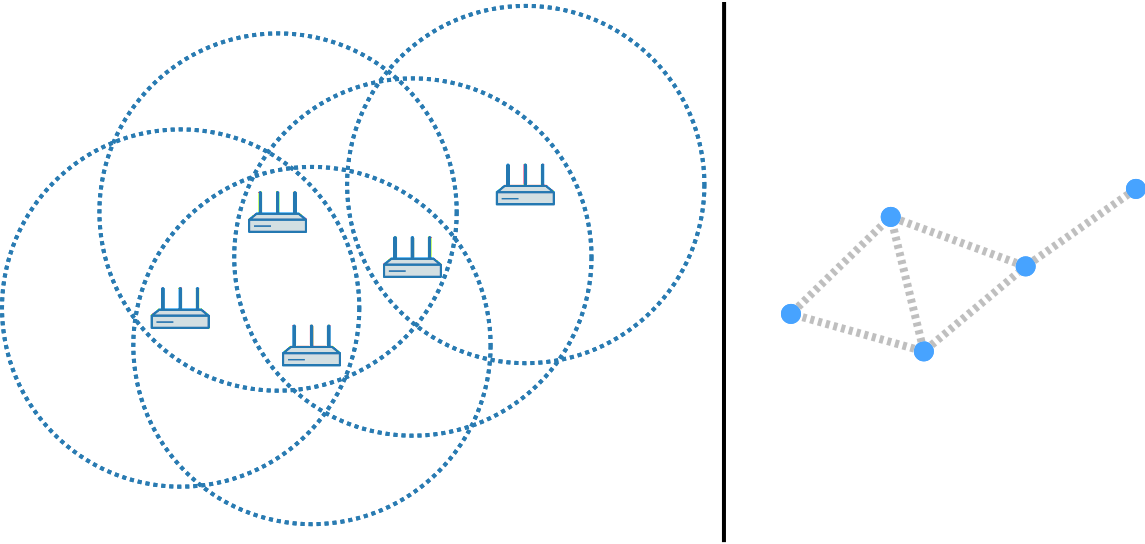
\includegraphics[width=1\columnwidth]{figures/unit-disk-graph}
    \caption{Creation of an unit disk graph from the receive range map of accesspoints}
    \label{fig:unit-disk-graph}
  \end{figure}
\section{\ac{CLICA}}
  The aim of \ac{CLICA}\cite{CLICA} is to minimize interference conflicts for a given unit disk graph preserving the connectivity.
  That means it takes the given network topology-graph as granted and tries to minimize the overall interference by resolving conflicts as much as possible.
  It takes the following parameters as input:
  \begin{itemize}
   \item Unit disk graph
   \item Number of radios at each node and total number of channels available
   \item Interference conflicts in form of a conflict graph
  \end{itemize}

  CLICA's mode of operation is described by \cite{overview_caa} as follows:
  \begin{quote}
    \begin{itemize}
      \item Randomly assign a node \(v\) the highest priority, then assign other
	nodes priorities decreasing in the order obtained by depth.
      \item While traversing the nodes in the decreasing order of their
	priorities obtained above, assign channels to the incident links
	of these nodes. The operation of assigning a channel to a link
	includes assigning this channel to both a radio at this node and
	a radio at the neighbor node. Then, the priorities of unvisited
	nodes are adjusted according to their degree of flexibility, which
	is the number of channels that a node can choose from without
	breaking the connectivity preservation. Essentially, the nodes
	with a lower degree of flexibility will have their priorities
	increased so that they are visited earlier in the later steps.
      \item When picking a channel in the above step, a node v1 picks
	a channel for its incident link (\(v_1\) , \(v_2\) ) in a greedy manner: a
	locally optimal choice is made by selecting the channel that
	minimizes the maximum link conflict weight among all links
	that can interfere with link (\(v_1\) , \(v_2\) ). After a channel is assigned
	to a link, the conflict graph is updated to reflect the new link conflict weights.
    \end{itemize}
  \end{quote}
  
  The reason why we decided not to use this algorithm is that \ac{CLICA} only tries to minimize interference by assigning channels the best way possible for a given
  unit disk graph, which is basically each possible connection. For a highly connected network topology like \ref{fig:graphseen} this would lead to suboptimal results
  as it does not try to select just some of those connections. The restriction to use only the best and absolutely neccessary links is a vital part in order to 
  further decrease interference as much as possible for such a topology.
\section{\ac{INSTC}}
  As pointed out by \cite{overview_caa}, INSTC \cite{INSTC} is similar to \ac{CLICA} with a few alterations, which is why we do not want to explain it here in detail and rather focus on
  its differences. They introduce \ac{LCI} which for a link represents the number of links which interfere with this link \cite{overview_caa} and serves as a measure of 
  interference. Additionally they accept \(k\) as input parameter which results in a \(k\)-connected Graph as outcome to make the topology resilient to node failures.
  Although this feature would come in handy for our survival path requirement, it does not match our failing scenario of a single link at a time instead of a whole node outage.
  Consequently the resulting network topology has a higher grade of connectivity than it needs to have and therefore conversely affects overall throughput since a higher
  node connectivity leads to less useable different channels. Additional to the weaknesses of \ac{CLICA}, they also require the number
  of radio modules per accesspoint to be identical, which is not desireable for us as requirement analysis dictates the operability also for heterogenous networks where this
  restriction is not met. The LCI measure served as a basis for our edgescore calcuation in ~\ref{eq:edgescore}.
  
\section{\ac{BFS-CA}}
  input: unit disk graph
	 location of gateway
	 number of radios at each node and total number of channels
	 internal interference MCG
	 external interference
  Does: reduce internal and external interference
	assign channel to vertices MCG
	bfs by distance from gateway
	greedy by MCG + internal + external interference
  \cite{BFS-CA}
\section{\ac{CTA}}
  This algorithm works on the conflict graph for a given unit disk graph.
  Input: unit disk graph
	 conflict graph
  Does: reduce total network interference + interface constraint
	assign channels to vertices in conflict graph
	translated to Max K-cut problem + Tabu search
  \cite{CTA}

\begin{description}
 \item [Which solutions do already exist?]
 \item[How do those solutions work?]
 \item[Why can't / won't we use those?]
\end{description}